Este apéndice recoge distintas vistas de la pantalla principal de SocratiCode y las pantallas de gestión de contraseña y recuperación de acceso.

\paragraph{Versiones de la pantalla principal.}

La pantalla principal admite varias configuraciones según las necesidades del alumno en cada momento. La \autoref{fig:pantalla-ejemplo} muestra la vista completa con el \textit{sidebar}, el editor con código y salida y el chat con una conversación activa.

\begin{figure}[Vista completa]{fig:pantalla-ejemplo}{Vista completa de SocratiCode con los tres paneles activos y contenido en cada uno de ellos.}
    \centering
    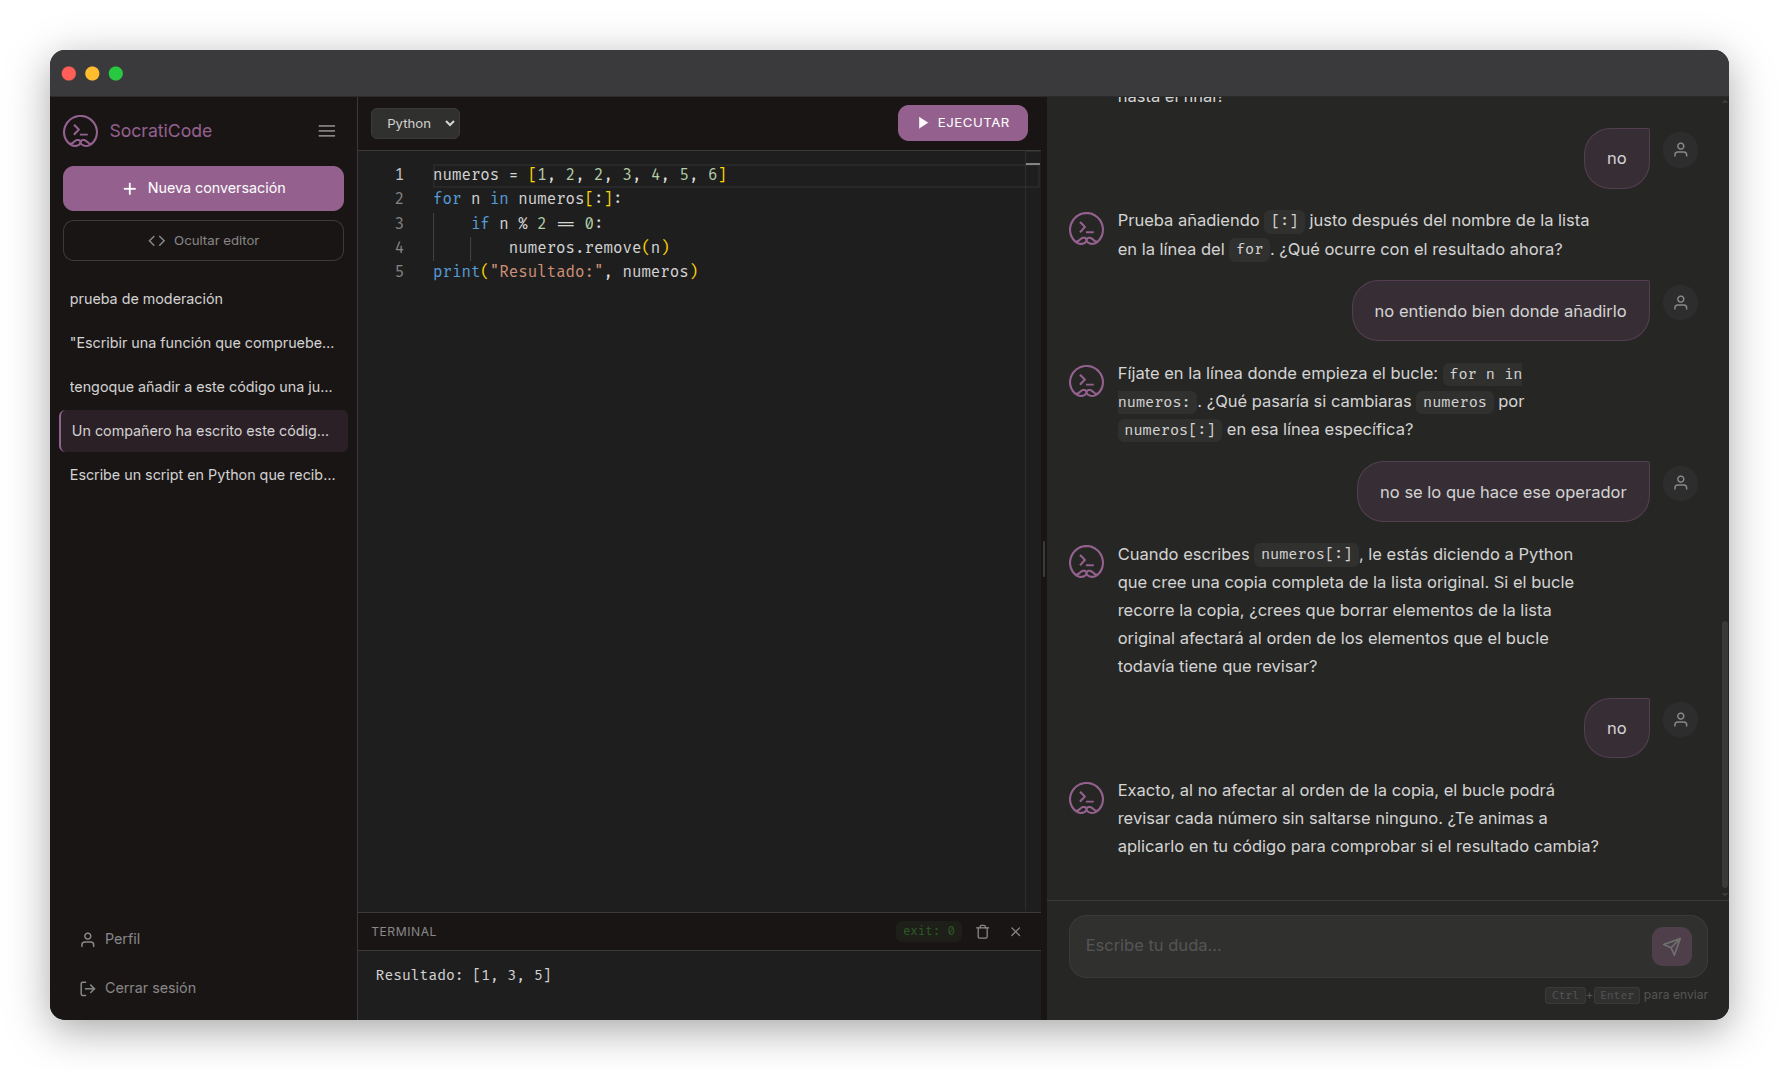
\includegraphics[width=\textwidth]{./pantallas/pantalla_ejemplo.png}
\end{figure}

Cuando el alumno quiere centrarse en el código, puede colapsar el \textit{sidebar}, que queda reducido a una franja estrecha en el lateral izquierdo. De este modo el editor y la terminal ganan espacio horizontal, tal y como se aprecia en la \autoref{fig:pantalla-centrado-codigo}.

\begin{figure}[Centrado en el código]{fig:pantalla-centrado-codigo}{Vista con el \textit{sidebar} colapsado para maximizar el espacio del editor y la terminal.}
    \centering
    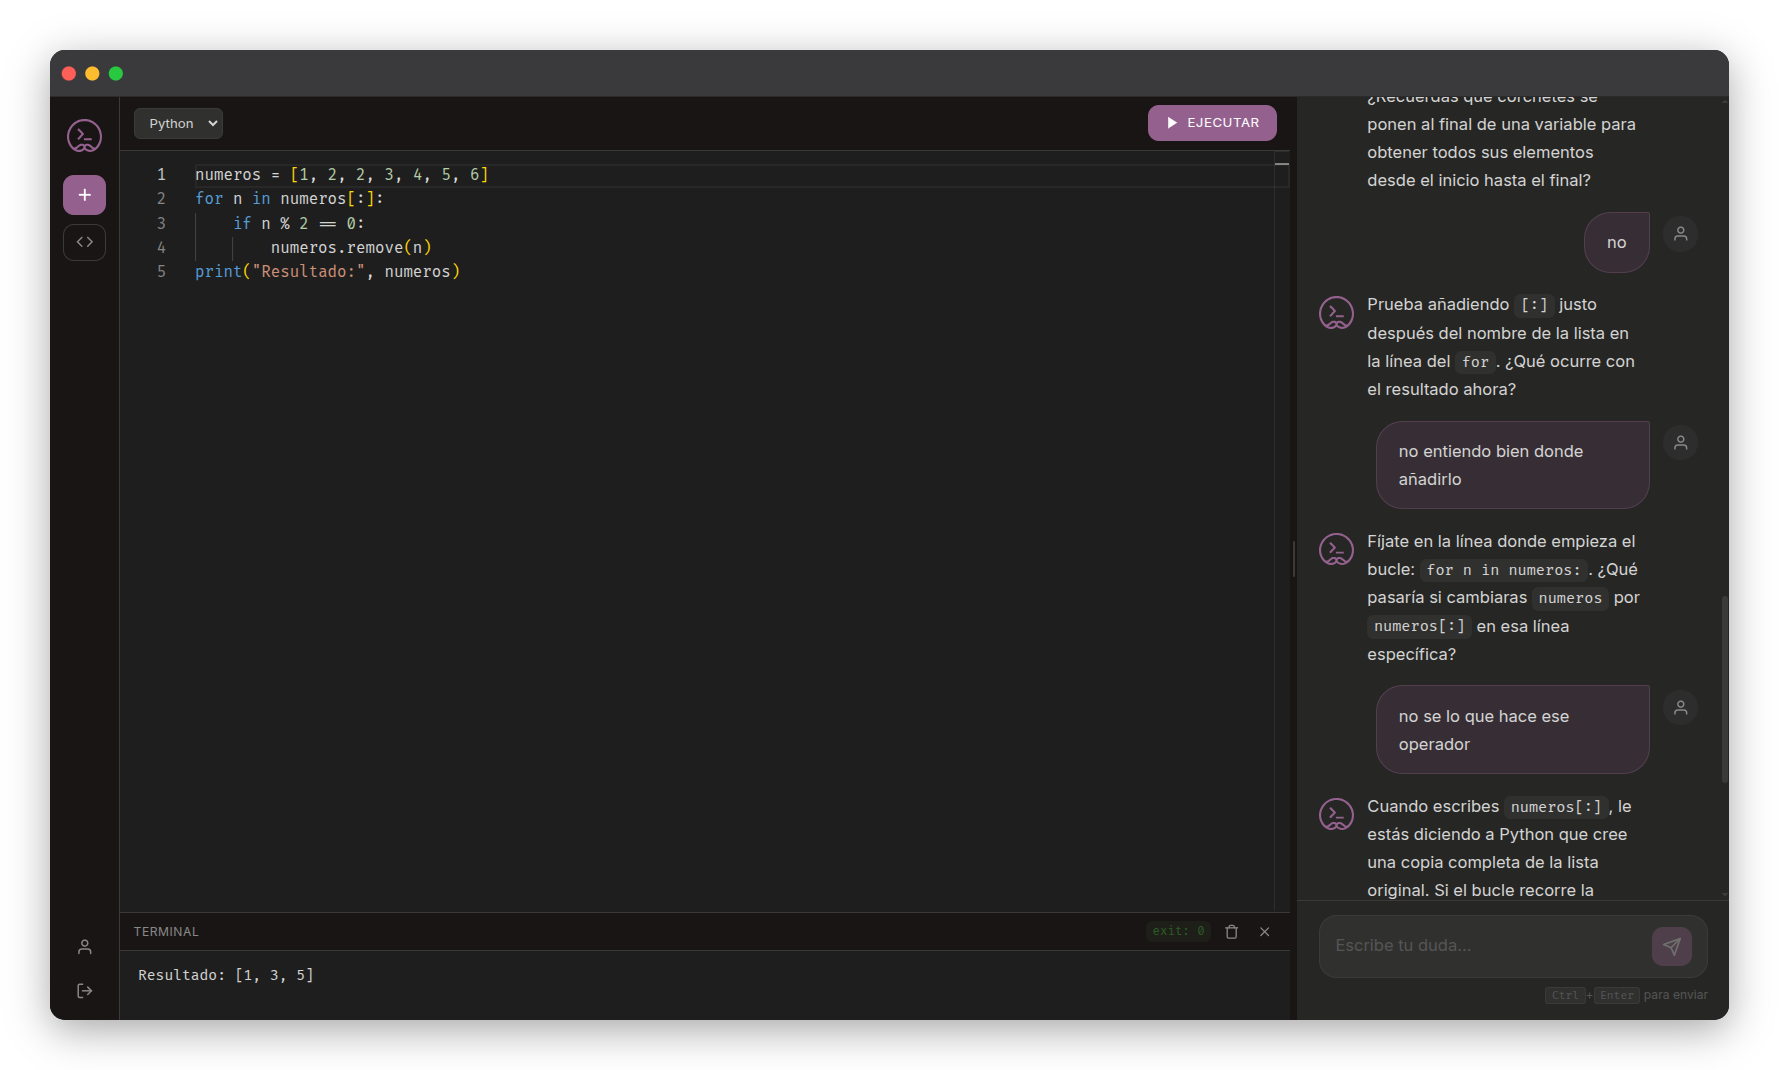
\includegraphics[width=\textwidth]{./pantallas/pantalla_centrado_codigo.png}
\end{figure}

Por el contrario, cuando la actividad es de carácter conceptual, el alumno puede ocultar el editor mediante el botón correspondiente. El chat pasa entonces a ocupar todo el espacio disponible junto al \textit{sidebar}, como se muestra en la \autoref{fig:pantalla-centrado-chat}.

\begin{figure}[Centrado en el chat]{fig:pantalla-centrado-chat}{Vista con el editor colapsado: el chat ocupa todo el espacio central.}
    \centering
    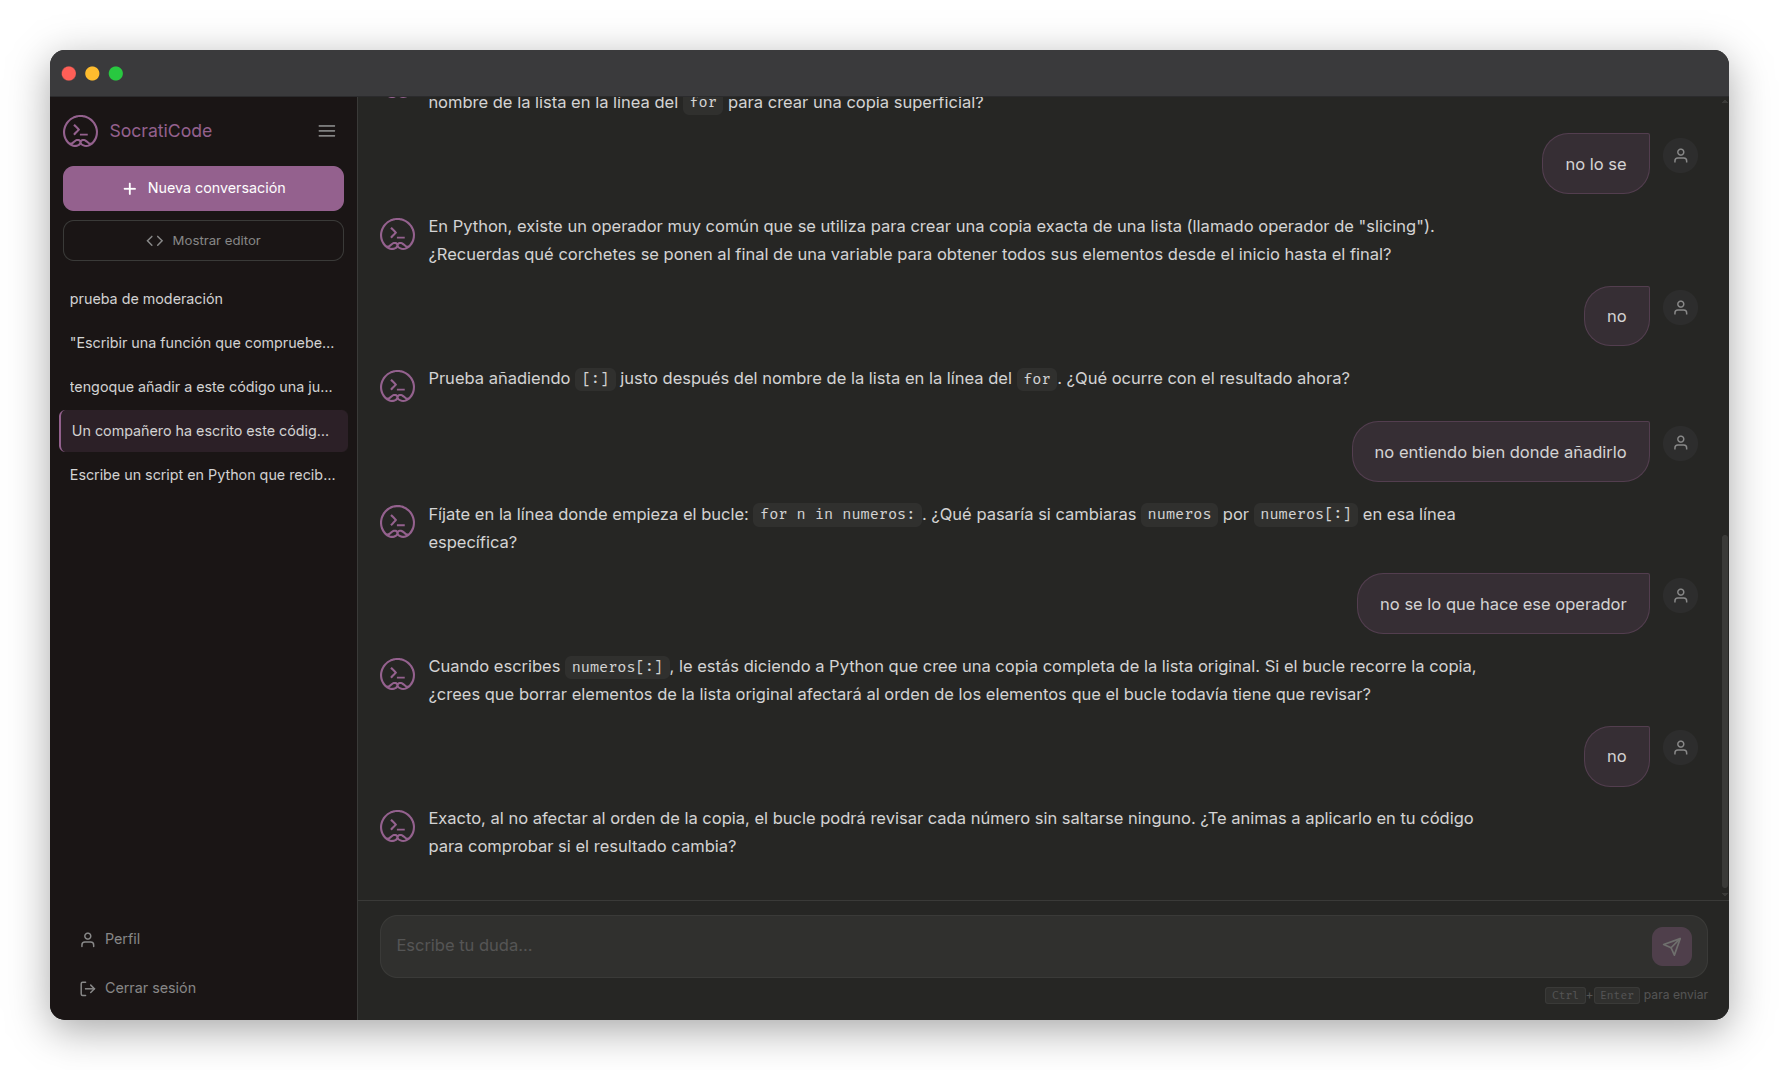
\includegraphics[width=\textwidth]{./pantallas/pantalla_centrado_chat.png}
\end{figure}

\paragraph{Cambio de contraseña.}

Desde la parte inferior de la pantalla de perfil el alumno puede establecer una nueva contraseña introduciendo la contraseña actual y la nueva dos veces para confirmarla. La \autoref{fig:cambio-contrasena} muestra este formulario.

\begin{figure}[Cambio de contraseña]{fig:cambio-contrasena}{Formulario de cambio de contraseña desde la pantalla de perfil.}
    \centering
    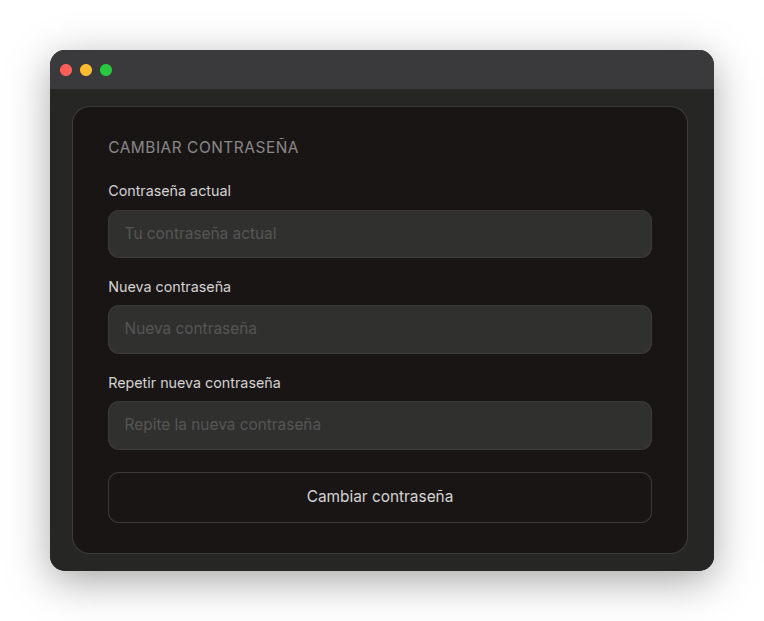
\includegraphics[width=0.6\textwidth]{./pantallas/pantalla_cc.png}
\end{figure}

\paragraph{Recuperación de contraseña.}

El flujo de recuperación de acceso consta de tres pasos. El usuario introduce su dirección de correo electrónico, recibe una confirmación de que el enlace ha sido enviado y, al acceder al enlace, establece una nueva contraseña. La \autoref{fig:recuperacion} recoge estas tres pantallas.

\begin{figure}[Recuperación de contraseña]{fig:recuperacion}{Pantallas del flujo de recuperación de contraseña: solicitud por correo, confirmación de envío y restablecimiento.}
    \centering
    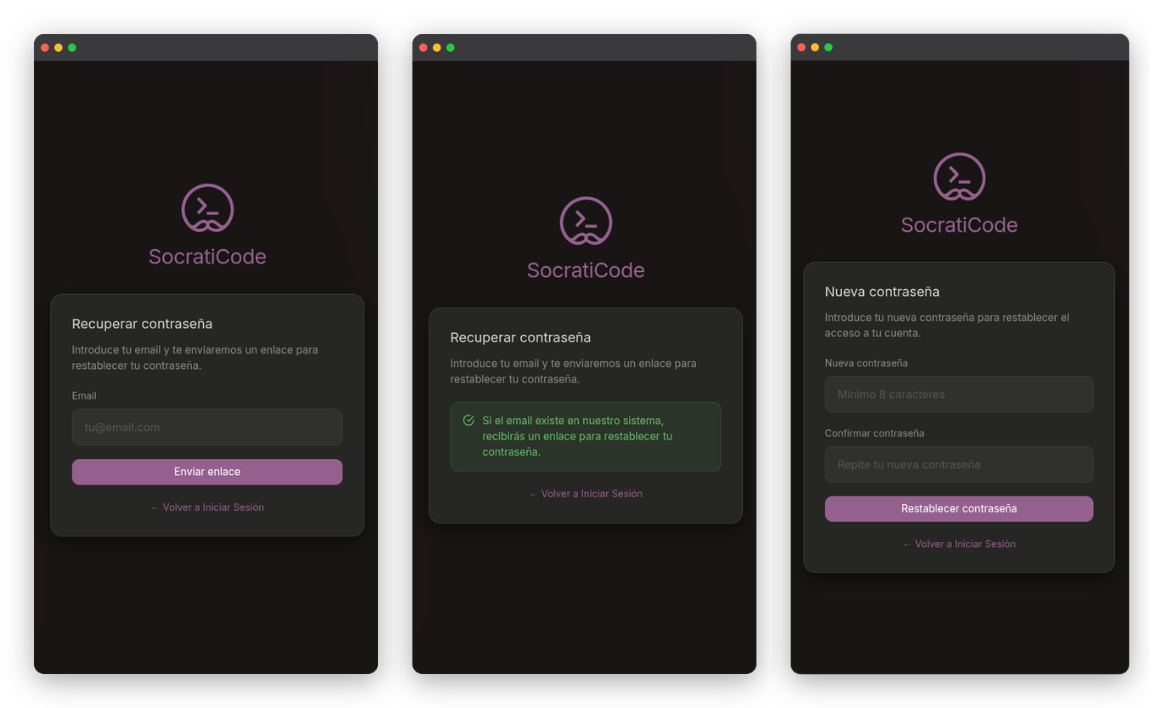
\includegraphics[width=\textwidth]{./pantallas/pantallas_recuperacion.png}
\end{figure}
